\documentclass[french, 11pt]{article} 

%=================================================
% Packages and New Commands
%=================================================

%===== Packages ==================================
%=================================================

\usepackage[utf8]{inputenc}

\usepackage[]{afterpage}
\usepackage[]{amsfonts}
\usepackage[]{amsmath, amssymb}
\usepackage[toc, page]{appendix}
\usepackage[french, english]{babel}
\usepackage[citestyle=verbose-trad2, bibstyle=numeric, sorting=nty]{biblatex}
\usepackage[]{blindtext}
\usepackage[]{booktabs}				% Better tables.
\usepackage[]{caption}
\usepackage[]{chngcntr}
\usepackage[]{csquotes}
\usepackage[]{enumitem}
\usepackage[]{etoolbox}
\usepackage[]{fancyhdr}				% Page headers package.
\usepackage[]{float}
\usepackage[T1]{fontenc}
\usepackage[]{fontspec}
\usepackage[]{gensymb}
\usepackage[a4paper, total={162mm,245mm}, top=28mm]{geometry}
\usepackage[]{graphicx}
\usepackage[]{hyperref}
\usepackage[]{lastpage}
\usepackage[]{layout}
\usepackage[]{listings}				% Code insert package.
\usepackage[]{lmodern}
\usepackage[]{lscape}
\usepackage[]{makecell}
\usepackage[]{mathtools}
\usepackage[]{mathrsfs}
\usepackage[]{mdframed}
\usepackage[]{multicol}
\usepackage[]{multirow}
\usepackage[nottoc]{tocbibind}
\usepackage[]{parskip}
\usepackage[]{pdfpages}
\usepackage[]{pgfplots}
\usepackage[]{soul}
\usepackage[]{subcaption}
\usepackage[]{titlesec}
\usepackage[normalem]{ulem}
\usepackage[]{url}
\usepackage[]{wrapfig}
\usepackage[]{xcolor}

%===== New Commands ==============================
%=================================================

% New command to create a blank page without it being counted on the total page count.
\newcommand{\blankpage}
{
	\null
	\thispagestyle{empty}
	\addtocounter{page}{-1}
	\newpage
}

\newcommand{\question}[1]
{
	\vspace{0.3cm}
	\begin{mdframed}[style=Question]
		#1
	\end{mdframed}
}

\newcommand{\CMDblock}[1]
{
	{\colorbox{black!15}{\texttt{#1}}}
}

\newcommand{\HESSo}{HES$\cdot$So\xspace}
\newcommand{\HESGe}{HES$\cdot$Ge\xspace}

\newcommand{\DocVersion}{1.3.2}

\newcommand{\DocTitle}{Projet Micro-contrôleurs}
\newcommand{\DocSubject}{Microcontrôleur et Périphériques}

\newcommand{\SubjectProfessor}{M. Tarik Garidi\xspace}

% Make \paragraph as a subsubsubsection
\makeatletter
\renewcommand{\paragraph}{\@startsection{paragraph}{4}{0ex}%
   {-3.25ex plus -1ex minus -0.2ex}%
   {1.5ex plus 0.2ex}%
   {\normalfont\normalsize\bibfont\bf}}
\makeatother

% Make \paragraph appear in TOC
\stepcounter{secnumdepth}
\stepcounter{tocdepth}

%=================================================
% Themes, Colors and Styles
%=================================================

\mdfdefinestyle{Question}{backgroundcolor = black!5, linecolor=black!10, linewidth=2pt}

%=================================================
% Packages Configuration
%=================================================

\hypersetup
{
	bookmarksopen=true,
	pdftitle="\DocTitle\ - \DocSubject",
	pdfauthor="Joachim Bach ; David Da Silva Marques",
	pdfsubject="Bachelor I.S.C",
	pdftoolbar=true,				% Toolbar hidden.
	pdfpagemode=UseOutlines,
	pdfstartview={Fit},				% Fits the width of the page to the window.
	pdfmenubar=true,
	pdfhighlight=/O,
	colorlinks=true,
	pdfpagelayout=OneColumn,
	pdffitwindow=false,
	linktoc=section,
	linkcolor=blue,
	citecolor=blue,
	urlcolor=blue,
}

\bibliography{Others/Bibliography.bib}

\AtEveryCitekey
{
	\clearfield{urldate}
}

%=================================================
% Document Details - Preamble
%=================================================

\title{\DocSubject}
\author{Joachim BACH ; David DA SILVA MARQUES}
\date{\today}

\makeatletter
\let\TheTitle\@title
\let\TheAuthor\@author
\let\TheDate\@date
\makeatother

\pagestyle{fancy}
\fancyhf{}
\lhead{ \textsc{HEPIA Genève} \\ \DocSubject}
\rhead{ \textsc{version} \DocVersion \\ \TheDate}
\cfoot{\thepage \hspace{0.1 mm} / \pageref*{LastPage}}

%=================================================
%=================================================
%=================================================
% Start Document
%=================================================
%=================================================
%=================================================

\begin{document}
	
	\selectlanguage{french}
	\normalsize
	
	\begin{titlepage}
		
		\centering
		\vspace*{2.0 cm}
		
		\includegraphics[scale = 1.50]{Images/00_HEPIA_Logo.png}\\[1.0 cm]
		
		\vspace{1.0 cm}
		
		\rule{\linewidth}{0.3 mm} \\[0.2 cm]
		{\Huge \textbf{\DocTitle}}\\
		\vspace{4 mm}
		{\huge \TheTitle}\\
		\rule{\linewidth}{0.3 mm} \\[1.2 cm]
		
		\textsc{\Large Bachelor I.S.C}\\[0.5 cm]
		
		\vspace{1.5 cm}
		
		\begin{minipage}{0.40\textwidth}
			
			\begin{flushleft}
				\Large\emph{Auteur(s) :}\\[0.2 cm]
				\Large\emph{}\\[0.2 cm]
				\Large\emph{}\\[0.2 cm]
				\Large\emph{}\\[0.2 cm]
				\Large\emph{Institution :}\\[0.2 cm]
				\Large\emph{Date :}\\[0.2 cm]
				\Large\emph{Version :}\\[0.2 cm]
				\Large\emph{Professeur-re :}\\[0.2 cm]
			\end{flushleft}
		
		\end{minipage}~
		\begin{minipage}{0.53\textwidth}
			
			\begin{flushright}
				\Large{Joachim Bach (22650667)}\\[0.2 cm]
				\Large{David Da Silva Marques (226449792)}\\[0.2 cm]
				\Large{Alejandro Escribano Martín (15315914)}\\[0.2 cm]
				\Large\emph{}\\[0.2 cm]
				\Large{HEPIA Genève}\\[0.2 cm]
				\Large{\TheDate}\\[0.2 cm]
				\Large{\DocVersion}\\[0.2 cm]
				\Large{\SubjectProfessor}\\[0.2 cm]
			\end{flushright}
		
		\end{minipage}
	
	\end{titlepage}
	
	\blankpage

    \section{Introduction}

    Dans le cadre du cours Microcontrôleur et Périphériques (MIPS), nous avons dû réaliser un projet. Celui-ci a pour but, et exigencem, de réunir l'ensemble des interfaces et fonctionnalités étudiées durant ce semestre.

    La contrainte principale est que nous devions utiliser deux carte MyLab2.

    Nous avions aussi pour contrainte d'utiliser au moins les interfaces suivantes:

    \begin{enumerate}
        \item CAN
        \item Écran avec texte
        \item Communication UART
        \item Dalle tactile
        \item SysTick/Timer
        \item Boutons
    \end{enumerate}

    \section{Notre projet}

    Le projet que nous avons choisis consiste en une sorte de manette de jeu pour jouer à Assetto Corsa. Une des deux cartes sert de volant, grâce à l'accéléromètre, avec des boutons pour accélérateur et frein. Les leds du dipswitch sont utilisé comme indicateur de compte-tours. L'autre carte sert de tableau de bord affichant la télémétrie du jeu et ayant un touchpad pour permettre quelques inputs supplémentaires.

    \section{Architecture}

    \begin{figure}[H]
        \centering
        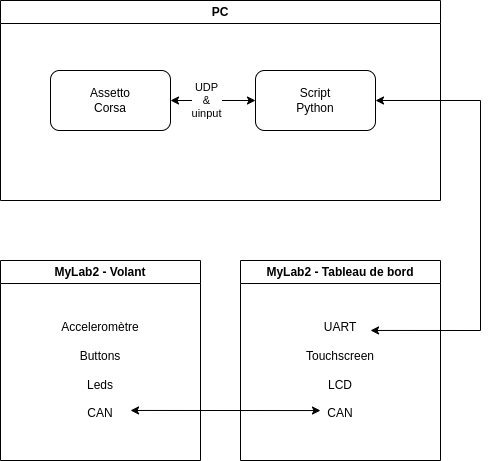
\includegraphics[width=0.95\textwidth]{architecture.drawio.png}
        \caption{Schéma de l'architecture}
    \end{figure}
        
        \subsection{PC}

        Du côté du PC, se trouve Assetto Corsa, un jeu de voiture, et un script python tournant en fond. Ce script python se charge de récupérer la télémétrie d'Assetto Corsa à travers un socket UDP. Il récupére les informations qui l'intéresse et les envoie sur l'UART vers le "Tableau de bord", autrement dit l'une des deux cartes. Ce cette même connexion UART, le script récupére les inputs sous formes de tableau de bytes depuis la carte. Ces informations sont ensuite transmis à une class "Gamepad" qui simule un périphérique qui est ensuite utiliser par le jeu comme un n'importe quel autre périphérique/manette/etc.


        \subsection{Volant}

        Le volant s'occupe de récuperer les valeurs de son accéléromètre et les convertirs en un angle. Il envoie en continu le résultat de ce calcul par CAN au tableau de bord. Quand on appuie sur le bouton A ou B, un message CAN est transmis immédiatement au tableau de bord aussi. Le volant reçoit sur le CAN, les RPM du moteur et la vitesse de la voiture. Ceux-ci seront affiché respectivement sur les leds des dipswitch et sur le lcd sous forme de cadrant avec une aiguille.

        
        \subsection{Tableau de bord}

        Le tableau de bord est la pièce central du projet, dans le sens où c'est cette carte qui sert d'intermédiaire entre le volant et le PC. Le tableau de bord reçoit à travers l'UART la télémétrie, dont il affiche l'accélérateur et le frein, mais aussi le lap time. Il retransmets ensuite la vitesse et les RPM au volant. De celui-ci il récupère la rotation et les boutons, qu'il stock dans un tableau local. Toutes les 20ms, il envoie alors ce tableau par la même connexion UART pour que le PC puisse interpréter les inputs. 

        \subsection{Matériel}    

        Pour ce projet nous avons donc besoin:

        \begin{enumerate}
            \item 1 PC avec Assetto Corsa et 1 script python permettant d'interfacé avec les cartes
            \item 2 MyLab2 + LPC1769
            \item 1 cable usb A -> micro-usb
            \item 1 cable CAN
            \item Câbles d'alimentation
        \end{enumerate}

    \section{Conclusion}

    Initialement il avait été prévu que les cartes soient utilisé en tant périphériques USB. Cependant il s'avère que c'est un protocol relativement sensibles et précis, rendant compliqué son implémentation dans un délai aussi court. Heureusement un plan de secours avait été prévu, utiliser un script python couplé à de l'UART pour la transmissions des données pour pouvoir simuler un périphérique logiciellement. Cependant cette solution n'est pas miraculeuse et ne fonctionne pas de manière stable.
